\section{Das Morlet-Wavelet}
\rhead{Morlet Wavelet}
Auch die reellen Fourierreihen haben das Problem, dass man Amplitude und Phase nicht separat betrachten kann, wenn man nur die Cosinus-Terme verwendet.
Dies liegt daran, dass Amplitude und Phase beim Cosinus gekoppelt sind,
\[
x = A\cos(\alpha) \quad\leftrightarrow\quad \alpha = \cos^{-1}\left(\frac{x}{A}\right).
\]
Erst durch die komplexe Schwingung 
\begin{align*}
	z(t) = Ce^{i\omega t} &= |C|e^{i\left(\omega t + \arg C\right)}
%	 &= |C|\left[\cos\left(\omega t + \arg C\right) + i \sin\left(\omega t + \arg C\right)\right]
\end{align*}
erhält man eine Basisfunktion, die mit
\[
	|z(t)| = |C| \quad \text{und}\quad
	\arg z = \arg \omega t + \arg C
\]
eine separate Betrachtung von Amplitude und Winkel erlaubt.
Diese Eigneschaft überträgt sich von den Basisfunktionen auf die Fouriertransformation.
Aufgrund der eulerschen Formel
\begin{equation}
	\cos(x) = \frac{e^{ix} + e^{-ix}}{2}\label{complex:euler}
\end{equation}
kann der Cosinus aus zwei komplexen Exponentialfunktionen mit inverser Frequenz dargestellt werden.
Besitzt ein Wavelet also negative Frequenz-Anteile, dann geht bei diesen Frequenzen die Eigenschaft der Separierbarkeit von Amplitude und Phase verloren.

\begin{figure}
	\centering
	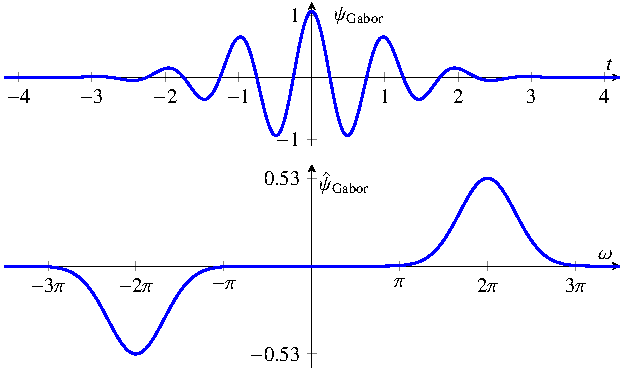
\includegraphics{papers/complex/images/gabor.pdf}
	\caption{Das Gabor-Wavelet für $\sigma = 2\pi$ \label{complex:gabor}}
\end{figure}

Ein geeignetes Wavelet benötigt folglich eine Fouriertransformierte, die bei negativen Frequenzen verschwindet.
Betrachten wir nun das Gabor-Wavelet
\[
	\psi = c_\sigma e^{-\frac{t^2}{2}}\left(\cos\left(\sigma t\right) - \kappa_\sigma\right),
\]
welches auch in Abbildung~\ref{complex:gabor} ersichtlich ist.
$c_\sigma$ und $\kappa_\sigma$ sind hierbei positive, reelle Konstanten, welche die Norm und die Zulässigkeitsbedingung~\eqref{cwt:zulaessig} korrigieren.
$\kappa_\sigma$ ist typischerweise sehr klein und wird oftmals einfach weggelassen.
Dieses Wavelet besitzt die dominante Frequenz $\sigma$ und ist durch die Gaus-Funktion in der Zeit lokalisiert.
Das Gabor-Wavelet eignet sich deshalb besonders gut, um einzelne Frequenzen in einem Signal zu finden.

Durch die Cosinus-Funktion besitzt das Gabor-Wavelet jedoch negative Frequenzen, wodurch eine isolierte Betrachtung von Amplitude und Phase unmöglich wird.
Dies möchten wir im Folgenden korrigieren.
Hierzu wechseln wir in den Fourierbereich.
Wir nutzen aus, dass die Fouriertransformierte einer Gaus-Kurve wieder eine Gauskurve ist,
\[
	\mathcal{F}\left\lbrace e^{-\alpha x^2} \right\rbrace 
	= \frac{1}{\sqrt{2\alpha}}e^{- \frac{\omega^2}{4\alpha}},
\]
und dass die Multiplikation im Zeitbereich zur Faltung im Frequenzbereich wird.
Zudem verwenden wir die Eulerformel~\eqref{complex:euler}.
Die Fouriertransformeirte des Gabor-Wavelet wird hierdurch zu
\[
 \hat{\psi} = 
 c_\sigma e^{- \frac{\omega^2}{2}} * \left(
  \frac{1}{2}\delta(\omega - \sigma) +
  \frac{1}{2}\delta(\omega + \sigma) + 
  \kappa_\sigma\delta(\omega)
  \right).
\]
Hierbei bezeichnet $\delta(\omega)$ die Dirac-Distribution.
Hieraus lässt sich der negative Anteil des Cosinus leicht entfernen.
Zudem verdoppeln wir den Anteil der positiven Frequenzen (der Grund hierfür erschliesst sich im nächsten Kapitel).
Wir erhalten
\[
	\hat{\psi}^\ast = 
	c_\sigma e^{- \frac{\omega^2}{2}} * \left(
	\delta(\omega - \sigma) +
	\kappa_\sigma\delta(\omega)
	\right),
\]
und durch Rücktransformation in den Zeitbereich
\[
	\psi^\ast = 
	c_\sigma e^{- \frac{t^2}{2}} \cdot \left(
	e^{i\sigma t} +
	\kappa_\sigma
	\right).
\]
Dies ist ein alter Bekannter, das Morlet-Wavelet aus Gleichung~\eqref{cwt:morlet}.
Abbildung~\ref{complex:morlet} zeigt den Real- und Imaginärteil, so wie die Envelope des Morlet-Wavelets.
Die Unabhängigkeit der Amplitude und der Phase 
Die Envelope entspricht hierbei gerade dem Absolutwert.
Das Morlet-Wavelet eignet sich also besonder gut, um bestimmte Frequenzen in einem Signal zu lokalisieren.
Im nächsten Kapitel werden wir sehen, dass man aus jedem, reellen Wavelet eines konstruieren kann, welches eine separate Betrachtung von Amplitude und Phase ermöglicht.

\begin{figure}
	\centering
	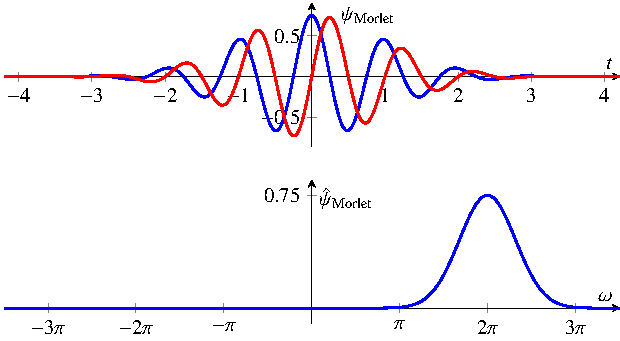
\includegraphics{papers/complex/images/morlet.pdf}
	\caption{Real- (blau) und Imaginärteil (rot) des Morlet-Wavelet für $\sigma = 2\pi$ \label{complex:morlet}}
\end{figure}